\documentclass[11pt]{article}

\usepackage[font=footnotesize]{caption}
\usepackage{float}
\usepackage{epsf}
\usepackage{epsfig}
\usepackage{subfigure}
% \usepackage{subfig}
\usepackage{latexsym}
%\usepackage{algorithm}
%\usepackage[noend]{algorithmic}
% \usepackage{color}
\usepackage{color, colortbl}
\usepackage{wrapfig}
% \usepackage{topcapt}
\usepackage{multirow}
\usepackage{tabularx}
\usepackage{hyperref}
\usepackage{xcolor}
\usepackage{mdwlist}
\usepackage{pdfpages} 
\usepackage{tabto}  
%\usepackage{color}
\newcommand{\lc}[1]{\textcolor{blue}{#1}}


\usepackage{amsmath, amsfonts, amssymb}
\usepackage[hmargin=1in,vmargin=1.2in]{geometry}
\usepackage{url}
\usepackage{multirow}
\usepackage[ruled,noline,linesnumbered]{algorithm2e}
\usepackage[bottom]{footmisc}
\usepackage{afterpage}
%\usepackage[caption=false]{caption}
\usepackage{eurosym}
\usepackage{enumitem}
% \usepackage{soul}
\usepackage{fancyhdr}
\usepackage{dashrule}
% \usepackage[stable]{footmisc}
% \usepackage{placeins}
% \setitemize{noitemsep,topsep=0pt,parsep=0pt,partopsep=0pt}
% \usepackage[utf8]{inputenc}
% \usepackage{gensymb}
\usepackage{rotating}
% \usepackage{tikz}
% \usepackage[firstpage]{draftwatermark} 

% \SetWatermarkText{DRAFT}
% \SetWatermarkScale{1}
% \SetWatermarkLightness{0}

% \interfootnotelinepenalty=80 
% \floatingpenalty=0\relax
\widowpenalty=1000
\clubpenalty=1000

\def\dec{{\texttt{UN Decade of the Oceans\ }}}
\def\dece{{\texttt{UN Decade of the Oceans}}}

\def\soc{{\texttt{SOCIB\ }}}
\def\soce{{\texttt{SOCIB}}}
\def\mit{{\texttt{MIT\ }}}
\def\mite{{\texttt{MIT}}}
\def\colo{{\texttt{Columbia\ }}}
\def\coloe{{\texttt{Columbia}}}
\def\ave{{\texttt{UAveiro\ }}}
\def\avee{{\texttt{UAveiro}}}
\def\inst{{\texttt{IH\ }}}
\def\inste{{\texttt{IH}}}
\def\proj{{\textbf{FRESNEL\ }}}
\def\proje{{\textbf{FRESNEL}}}
\def\met{{\textbf{METEOR\ }}}
\def\mete{{\textbf{METEOR}}}
\def\rx{{\texttt{T-REX\ }}}
\def\rxe{{\texttt{T-REX}}}
\def\eut{{\texttt{EUROPA$_2$\ }}}
\def\eu{{\texttt{EUROPA\ }}}
\def\eue{{\texttt{EUROPA}}}
\def\nd{{\texttt{NDDL\ }}}
\def\nde{{\texttt{NDDL}}}
\def\du{{\texttt{DUNE}\ }}
\def\due{{\texttt{DUNE}}}
\def\nep{{\texttt{NEPTUS}\ }}
\def\nepe{{\texttt{NEPTUS}}}
\def\rip{{\texttt{Ripples}\ }}
\def\ripe{{\texttt{Ripples}}}
\def\imc{{\texttt{IMC}\ }}
\def\imce{{\texttt{IMC}}}
\def\hub{{\texttt{HUB}\ }}
\def\hube{{\texttt{HUB}}}
\def\mse{{\texttt{MSEAS}\ }}
\def\msee{{\texttt{MSEAS}}}
\def\naz{{Nazar\'{e}\ }}
\def\naze{{Nazar\'{e}}}


\interfootnotelinepenalty=10000

\def\etal{{et al.\/}}
\def\eg{e.g., }
\def\ie{{i.e.,\ }}
\def\etc{{etc.\ }}
\def\situ{{in situ \/}}
\def\PN{{\emph{PN} }}

\definecolor{Gray}{gray}{0.6}

\newlength{\doublespacelength}
\setlength{\doublespacelength}{\baselineskip}
\addtolength{\doublespacelength}{0.5\baselineskip}
\newcommand{\doublespace}{\setlength{\baselineskip}{\doublespacelength}}

\newlength{\singlespacelength}
\setlength{\singlespacelength}{\baselineskip}
\newcommand{\singlespace}{\setlength{\baselineskip}{\singlespacelength}}


\newlength{\savedspacing}
\newcommand{\savespacing}{\setlength{\savedspacing}{\baselineskip}}
\newcommand{\restorespacing}{\setlength{\baselineskip}{\savedspacing}}

\setlength{\parskip}{0pt}
\setlength{\parsep}{0pt}
\setlength{\headsep}{0pt}
\setlength{\topskip}{0pt}
\setlength{\topmargin}{0pt}
\setlength{\topsep}{0pt}
\setlength{\partopsep}{0pt}

\newtheorem{definition}{Definition}
\newcommand{\hide}[1]{}
\newcommand{\com}[1]{{\color{red}{#1}}}
\newcommand{\kc}[1]{{\color{blue}{#1}}}
\newcommand{\wh}[1]{{\color{white}{#1}}}

\newcounter{quotenumber}

\newenvironment{numquote}{%
    \begin{enumerate}%
     \setcounter{enumi}{\value{quotenumber}}%
     \color{darkgray}
    \item \begin{quote}%
}{%
    \end{quote}%
    \setcounter{quotenumber}{\value{enumi}}
    \end{enumerate}%
}%

\makeatletter
\def\myitem{%
   \@ifnextchar[ \@myitem{\@noitemargtrue\@myitem[\@itemlabel]}}
\def\@myitem[#1]{\item[#1]\mbox{}}
\makeatother



\newcommand\blankpage{%
    \null
    \thispagestyle{empty}%
    \addtocounter{page}{-1}%
    \newpage}

\setcounter{secnumdepth}{0} 

\let\oldthebibliography\thebibliography
\let\endoldthebibliography\endthebibliography
\renewenvironment{thebibliography}[1]{
  \begin{oldthebibliography}{#1}
    \setlength{\itemsep}{0em}
    \setlength{\parskip}{0em}
}
{
  \end{oldthebibliography}
}
% \linespread{0.98}
\parskip 0.1cm


\title{On Model-Driven Ocean Exploration}

%Robotics Assimilation

\author{
Renato Mendes\textsuperscript{1,2,3,*},
Lucrezia Bernacchi \textsuperscript{1},
Leonardo Azevedo \textsuperscript{4},
Ana F. Duarte \textsuperscript{4},\\
Marina Cunha \textsuperscript{5},
Clara Rodrigues \textsuperscript{5},
João Borges de Sousa \textsuperscript{1,3},
João Vitorino \textsuperscript{7},\\
Ajit Subramaniam \textsuperscript{6},
Fernando Esteves \textsuperscript{8},
Kanna Rajan \textsuperscript{8,1}
\\
\\
\textsuperscript{1}{\scriptsize Laboratório de Sistemas e Tecnologia Subaquática (LSTS), Faculdade de Engenharia da Universidade do Porto, Portugal}\\
\textsuperscript{2}{\scriptsize +ATLANTIC CoLAB, Lisboa, Portugal}\\
\textsuperscript{3}{\scriptsize Laboratório Associado de Energia, Transportes e Aeronáutica (LAETA), Porto, Portugal}\\
\textsuperscript{4}{\scriptsize Centro de Recursos Naturais e Ambiente (CERENA), Instituto Superior T\'{e}cnico, Universidade de Lisboa, Lisboa, Portugal}\\
\textsuperscript{5}{\scriptsize Universidade de Aveiro, Portugal}\\
\textsuperscript{6}{\scriptsize Lamont-Doherty Earth Observatory, Columbia University, New York}\\
\textsuperscript{7}{\scriptsize Instituto Hidrogr{\'a}fico Lisboa, Portugal}\\
\textsuperscript{8}{\scriptsize RAND Corporation, Washington D.C.}\\
\textsuperscript{*}\texttt{{\scriptsize renato.mendes@colabatlantic.com}}
}
\date{} 
\begin{document}

\maketitle
\section{Introduction}
% 1000-1500 words

%Coastal zones

The coastal ocean, the marine area extending from the coastline to the
continental slope, encompassing the continental shelf, constitutes one
of the most dynamic and complex regions of the ocean. These areas are
characterized by highly variable forcing mechanisms, intricate
topographies, and coastline geometries. They are forced by a wide
range of physical and biogeochemical processes which occur across
diverse spatial and temporal scales. They are among the most
productive and economically significant areas of the world’s oceans,
benefiting from terrestrial inputs via river discharges and nutrient
renewal driven by upwelling processes. As a result and in part,
coastal areas concentrate a great proportion of human maritime
activities, from fisheries and offshore aquaculture to renewable
energy exploitation. Moreover, the coastal ocean acts as an interface
between deep-ocean processes and coastal environment, modulating how
large-scale phenomena — such as climate-driven changes or extreme
weather events — impact coastal populations. It also regulates, for
example, how anthropogenic influences originating on land are
redistributed and affect marine ecosystems.

The complex interplay between physical, chemical, and biological
processes in the coastal ocean can rapidly amplify or modulate the
impacts of extreme events such as storms, flooding, or pollution
incidents. Furthermore, the coastal ocean serves as a key interface
where large-scale oceanic and atmospheric changes manifest their
consequences for coastal ecosystems. Accurately forecasting the state
of the coastal ocean is therefore essential not only for safeguarding
environmental and economic interests, but also for enhancing
resilience to climate variability, natural hazards, and human-induced
pressures.  Achieving this, however, remains a major scientific and
technological challenge, given the high variability, rapid dynamics,
and observational constraints inherent to these regions.

Ocean models have become essential tools for predicting the ocean
state and underpin a wide range of societal applications, from climate
forecasting to pollution monitoring and resource management. However,
these models are inherently imperfect representations of complex
reality. Data assimilation techniques — where observational data are
integrated into models — play a critical role in correcting or
adjusting model errors and improving their forecasting
capabilities. Yet, the success of data assimilation depends heavily on
the availability, quality, and relevance of observations.

Observations of the ocean are obtained through multiple sources.
Satellite remote sensing offers extensive spatial coverage but is
limited to surface measurements with usually low spatial resolution
and often compromised by atmospheric conditions. In situ observations,
whether from ships, moorings, or drifting platforms, provide higher
accuracy but suffer from limited spatial and temporal coverage, high
operational costs, and logistical constraints — particularly high in
coastal regions. Recent technological advances have enabled the use of
autonomous underwater vehicles (AUVs) and other robotic platforms,
offering flexible, mobile, and increasingly autonomous means of
sampling ocean properties with high spatiotemporal resolution and low
logistic footprint
\cite{das10,das11b,olaya12,graham12,jdas13,das15,sousa16,fossum18,fossum19,fossum19b}.

However, even with these new tools, efficiently gathering the
\textit{right} data remains a complex challenge. AUVs are constrained
by endurance, communication bandwidth, and operational risks such as
high currents and bathymetry. Meanwhile, the ocean itself remains
highly dynamic and unpredictable, with key processes often evolving
faster than traditional sampling strategies can capture. This opens
the door to adaptive sampling strategies, where observation efforts
are guided by model outputs and uncertainty estimates to maximize the
relevance of collected data. Adaptive sampling represents a
fundamental shift: instead of executing pre-planned missions,
autonomous vehicles dynamically prioritize areas for observation. One
approach that we articulate here is combining model predictions with
adaptive AUV sampling. Doing so combines predicted model uncertainties
in comparison with prior data assimilation process with availabe
obervations. Model forecasts identify where uncertainty is highest or
where new observations are expected to have the greatest impact in
reducing forecast errors. Vehicles are then directed to sample these
areas, and their data are in turn assimilated back into the models,
generating improved forecasts for subsequent adaptive planning as a
virtuous cycle.

%data-cycle
Doing so closes a critical feedback loop between models and
observations; model prediction generates a forecast and associated
uncertainty field while adaptive sampling targets areas of maximum
predicted uncertainty. Data assimilation from these regions of high
uncertainty are then incorporated into the model such that new
predictions benefit from improved in-situ data, closing the loop.

\begin{figure}
    \centering
    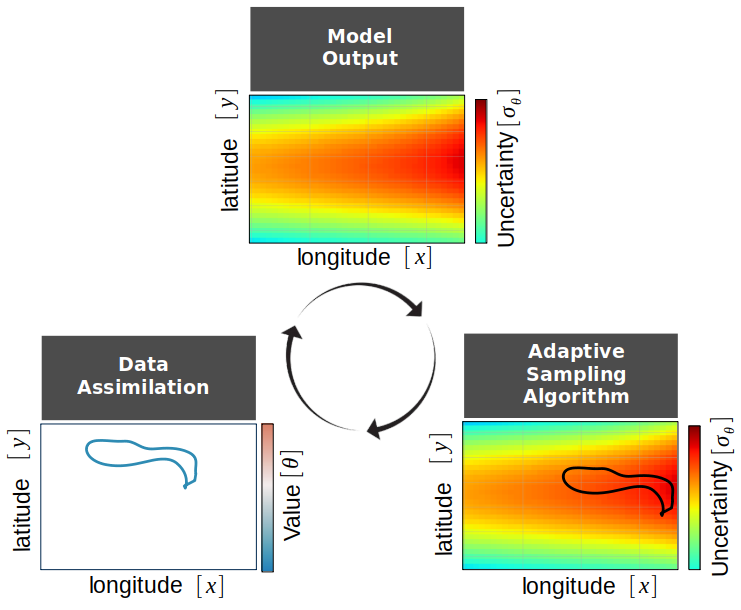
\includegraphics[width=.7\linewidth]{fig/data_cycle.png}
    \caption{Enter Caption}
    \label{fig:enter-label}
\end{figure}

Such a \textit{data cycle} approach promises to significantly enhance
the skill of ocean forecasts, especially in the complex coastal
environment where processes occur over a wide range of scales and where
human and environmental stakes are high. It also has the potential to
improve operational efficiency by optimizing the deployment of costly
and resource-constrained observational assets.

% real-world gap
Yet, implementing such a system in the real world presents substantial
challenges. It demands high-resolution numerical models capable of
rapidly generating uncertainty projections, robust algorithms for
exploration under a range of constraints, reliable communication links
for mission updates, and assimilation frameworks able to integrate
heterogeneous, real-time data streams. Furthermore, the logistical risks
and communication limitations inherent to marine operations — low
bandwidth, intermittent connections, unpredictable weather conditions —
impose additional constraints on the practical execution of adaptive
sampling missions.

%impact
In this study, we address these challenges by implementing and
evaluating a complete data cycle — from model prediction, to uncertainty
projection, to adaptive sampling and data assimilation — in a coastal
ocean environment. The work was conducted within the framework of \proj
(\textbf{F}ield expe\textbf{R}iments for mod\textbf{E}ling,
a\textbf{S}similatio\textbf{N} and adaptiv\textbf{E} samp\textbf{L}ing),
a project specifically designed to explore and test model-driven robotic
exploration strategies. \proj provided the experimental setting and
operational assets to demonstrate how model-based uncertainty fields can
drive adaptive sampling missions aimed at improving ocean model
predictive skills. This work focuses on the underlying problem: how to
effectively close the loop between model predictions, observational
targeting, and data assimilation to enhance ocean forecasts in highly
dynamic coastal environments. The experimental results obtained within
\proj serve to illustrate and validate the proposed approach,
highlighting the practical benefits and challenges of real-world
adaptive ocean exploration.


% \textit{\textbf{-	Set the context and background of your study.}}
% \begin{itemize}
% \item Fresnel proposal context
% \item Data cycle idea
% \item Model predictions and uncertainties -$>$ Improve quality of Data gathering -$>$ data assimilation into models -$>$ better model predictions
% \item Point out the logistics difficulties of doing this in the sea (low bandwidth comms, risks, computing time, etc)
% \end{itemize}

% \textit{-	\textbf{Clearly state the objective and significance of your research.}}
% \begin{itemize}
% \item real-world experiment to close the data loop between better efficiency to get data to improve the Improved Ocean Model Predictions\
% \end{itemize}
% \begin{itemize}
%     \item present a figure showing that idea of loop/cycle
% \end{itemize}

\section{Study Area}

\begin{figure}[!t]
  \vspace{-0.5cm}
  \centering
  \subfigure[Map of Portugal and the study area highlighted with the
  red rectangle.]{\label{fig:po-map}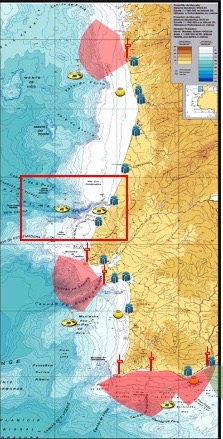
\includegraphics[scale=0.5]{fig/po-map.jpeg}}
  \hspace{+0.3cm}
  \subfigure[Zoomed in bathymetry showing the \naz canyon-Berlengas
  area (isobaths with depth in meters) and its environment including
  the placement of
  buoys.]{\label{fig:domain}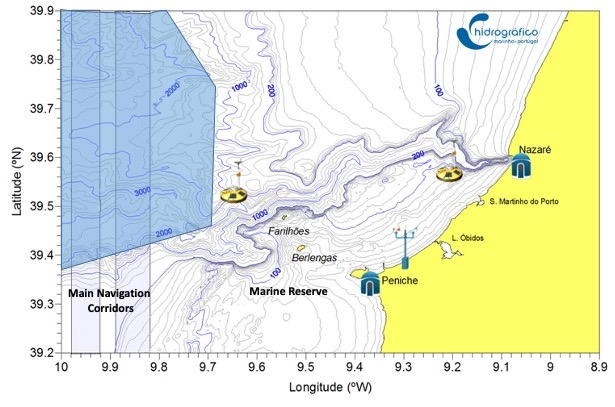
\includegraphics[scale=0.55]{fig/domain.jpg}}
  \caption{\subref{fig:po-map} \& \subref{fig:domain} show detailed
    views of the study area for \proj off the coast of mainland
    Portugal. The \naz Canyon is a significant feature of this area
    and a driver for the bio-geophysics of the domain.}
  \label{fig:studyarea-1}
\end{figure}

The study was conducted in the coastal ocean off central Portugal,
focusing on the region influenced by the \naz Canyon (39.2$^{\circ}$
-39.9$^{\circ}$N) (Fig. \ref{fig:studyarea-1}) in the Fall of
2024. While the experiment considered the measurable impact of model
driven robotic sampling to both the bio-geochemistry of the the canyon
region, this manuscript is focused on the implications of such
\emph{sample-assimilate-predict-direct} loop closure
(Fig. \ref{fig:loop-closure}).

% Added the text above to ensure that the reader knows other aspects of
% the experimemnt were NOT covered here. 


\begin{wrapfigure}{!h}{2.75in}
  \centering
 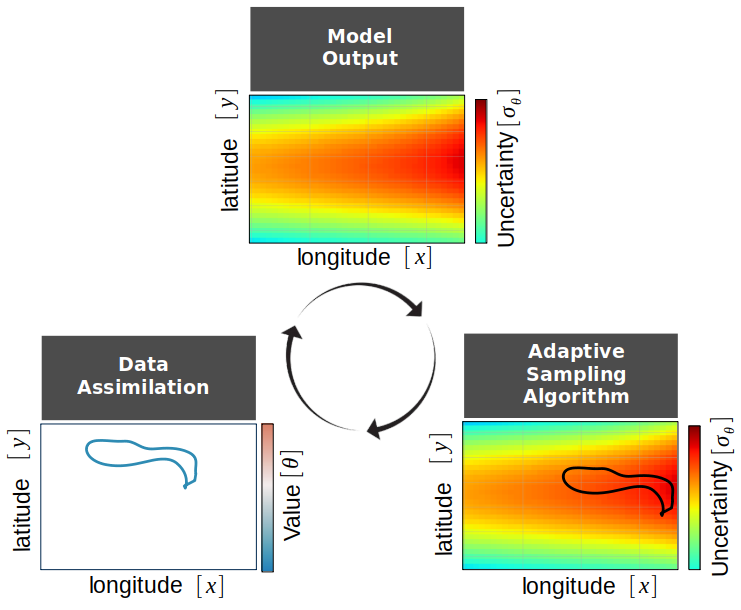
\includegraphics[scale=0.2]{fig/data_cycle.png}
  \caption{\proj attempts to close the
    \emph{sample-assimilate-predict-direct} loop using data obtained
    from robotic vehicles assimilated into a model which generates a
    prediction which in turn targets where the robotic vehicles can be
    repositioned to better address model uncertainty.}
  \label{fig:loop-closure}
\end{wrapfigure}


Implementing such a system in the dynamic real world of the coastal
region presents substantial challenges requiring high-resolution
numerical models capable of rapidly generating uncertainty
projections, robust algorithms for exploration under a range of
constraints, reliable communication links for mission updates, and
assimilation frameworks able to integrate heterogeneous, real-time
data streams. Furthermore, the logistical risks and communication
limitations inherent in marine operations — low bandwidth,
intermittent connections, unpredictable weather conditions — impose
additional constraints on the practical execution of adaptive sampling
missions.

The \naz area is shaped by strong topographic contrasts, including the
transition from the wide Estremadura Plateau to the narrower shelf to
the north, the long and narrow \naz submarine canyon that incises the
shelf and extends more than 200 km offshore, and the Berlengas
archipelago, a UNESCO Biosphere Reserve with high ecological
value. These features contribute to enhanced biological productivity
and biodiversity, and strongly modulate physical and biogeochemical
processes in the region.

Freshwater inputs from major rivers, such as the Tagus, have only a
limited direct impact on the area. In contrast, smaller rivers and the
\'{O}bidos lagoon can episodically deliver low-salinity, nutrient-rich
plumes to the shelf. Circulation is controlled by seasonal wind
forcing associated with the Azores High, with persistent
upwelling-favorable northerly winds in summer and frequent downwelling
episodes in winter under southerly winds. The interplay between canyon
topography, shelf circulation, and atmospheric forcing generates
complex mesoscale dynamics, intensified tidal currents, and internal
wave activity that promote strong vertical mixing and cross-shelf
exchanges \cite{martins10,quaresma07}.

The combination of sharp bathymetric gradients, variable forcing, and
rich physical–biogeochemical interactions makes the \naz Canyon region
an ideal natural laboratory to test adaptive observation
strategies. In particular, its dynamic environment posed both
opportunities and challenges for the \proj experiment, providing a
representative coastal setting in which to evaluate how model-based
uncertainty projections can guide adaptive sampling and assimilation
to improve ocean model predictive skill.

\section{Methods}
\label{sec:methods}


Our methodology is based on the implementation of a complete data cycle
to enhance model predictions in a coastal ocean domain through robotic
adaptive sampling and data assimilation. The approach consists of three
fundamental steps, executed iteratively on a daily basis:

\begin{description}

\item[Model Forecast and Uncertainty Projection]: A numerical ocean
  model provides a daily one-step forecast $\hat{\theta}(k+1, x, y)$
  of a target oceanic variable $\theta$, along with an associated
  uncertainty field $\sigma_{\hat{\theta}}(k+1, x, y)$, where $k$
  represents the current day and $(x, y)$ denote the geographical
  coordinates.  These outputs are organized into discrete spatial
  maps, $M_{\hat{\theta}}(x, y)$ and
  $M_{\sigma_{\hat{\theta}}}(x, y)$, representing, respectively, the
  predicted state and its uncertainty over a predefined grid covering
  the study area.
    
\item \textbf{Target Sample Planning}: Using the uncertainty map
  $M_{\sigma_{\hat{\theta}}}(x, y)$ as input, a targeted sampling
  algorithm determines the set of trajectories for a fleet of $N$ AUVs
  for the next operational cycle. The goal is to maximize the
  accumulated uncertainty sampled along the vehicle paths, while
  satisfying vehicle-specific constraints. The planned trajectories
  are transmitted to the vehicles for execution.

\item \textbf{Data Collection and Assimilation}: Throughout the
  operational period, each AUV collects measurements of the target
  variable $\theta$ along its assigned path. After the mission is
  completed, the collected measurements are assimilated into the
  numerical model using an appropriate data assimilation scheme. This
  updated model state serves as the new initial condition for the next
  forecasting cycle, closing the loop.

\end{description}

While previous efforts have concentrated on a form on embedded
automated decision-making on AUVs
\cite{mcgann08a,mcgann08b,ryan10,py10,Das-2010-637,das10,olaya12,rajan12}
to demonstrate adaptive sampling, here we AUV trajectories are defined
by human-in-the-loop decisions apriori, with adaptation focused on
deployment based on $M_{\sigma_{\hat{\theta}}}(x, y)$. No automated
decisions were made on the AUVs. Loop closure in this work, refers to
the \emph{sample-assimilate-predict-direct} process as shown in
Fig. \ref{fig:loop-closure}.

\subsection{Model Forecast and Uncertainty Projection}

Sampling strategies rely on timely information about the spatial
variability of ocean properties. However, conventional numerical ocean
models are computationally intensive, and their runtime makes them
impractical for use in near-real-time mission planning \kcomment{Need
  a citation here}. While similar assimilation cycles could, in
principle, be implemented directly within deterministic numerical
models, this would require either substantially higher computational
resources or larger temporal horizons. As a more practical
alternative, we employ geostatistical stochastic sequential simulation
as a computationally efficient surrogate, producing short-term spatial
predictions of ocean temperature together with estimates of spatial
uncertainty \cite{deutsch1992}. This approach captures the essential
variability of local ocean dynamics, based on calibrated dynamic ocean
models, at a fraction of the computational cost of full numerical
models, while remaining flexible enough to assimilate new in situ
observations quickly \cite{Duarte2025} and coherent with the scope of
the work approach.\kcomment{But what do we loose in turn? Resolution?
  Need to state that.}

The methodology relies on ensembles of geostatistical realizations,
each representing a state of the ocean temperature field conditioned
by \emph{a priori} deterministic ocean models \cite{CMEMS2017} and
direct observations. By computing the pointwise standard deviation
across the ensemble, we obtain spatial uncertainty maps that highlight
regions where predictions are less constrained and/or more variable
and potentially more informative for sampling. These maps serve as the
basis for identifying areas where new measurements are expected to
maximize the reduction of forecast error. In the field application
example shown here, the geostatistical realizations are produced using
direct sequential simulation \cite{soares2001direct}, a stochastic
method that draws values from conditional probability distributions
defined by kriging estimates and variances and conditioned to existing
direct measurements and a spatial covariance matrix. The continuity of
the temperature field in space and time is characterized by variogram
models fitted to long-term calibrated ocean model data from
E.U. Copernicus Marine Service (CMS) \cite{CMEMS2017}. At each depth
of the numerical ocean model, geostatistical simulations are carried
out independently, using a moving temporal window of fourteen previous
\kcomment{why 14? Where did this specific number come from?}  days as
conditioning data (i.e., experimental data) to predict the subsequent
day. This sliding-window strategy strikes a balance between forecast
skill and computational feasibility, and can be adapted according to
the complexity of the oceanographic conditions.

The ensemble of realizations provides both a forecast of ocean
temperature and a quantitative assessment of the prediction
uncertainty.  By updating the forecasts with new AUV measurements
through sequential assimilation, the method progressively refines the
temperature field while maintaining consistency with prior model
dynamics. The resulting forecasts and uncertainty maps form the input
for the target sampling algorithm, guiding the allocation of AUV
trajectories towards regions of greatest expected information
gain. More details about the model, its development, and application
during the \proj experiment can be found in \cite{Duarte2025}.

\subsection{Target Sampling Algorithm}

The adaptive sampling problem here is posed as the design of vehicle
trajectories that maximize information gain
\cite{eidsvik2015,fossum18} extracted from a model-derived uncertainty
map, while satisfying operational AUV constraints. Each day, the
models provide both a forecast field and its associated uncertainty
distribution, which together define the reward landscape for the
planner. The task is then to generate, for each vehicle, a path
composed of waypoints that accumulates the highest possible
uncertainty values.

To address this, the problem is cast as a graph theoretic problem. The
spatial uncertainty map is first pre-processed to remove obstacles and
smoothened to highlight large-scale features. Candidate waypoints are
then identified from the map and used to build a weighted graph, where
nodes carry a reward proportional to their uncertainty value and edges
represent travel costs. The trajectory planning task is posed as a
vehicle routing problem where routes must balance the rewards obtained
from visiting nodes with associated costs of traveling between them
\cite{vidal2013,toth2014vehicle}. By solving this, the algorithm
returns a set of near-optimal trajectories that prioritize regions of
greatest uncertainty, while ensuring vehicle endurance and safety
constraints. This provides a principled way of steering autonomous
platforms toward the most informative sampling locations, forming a
key component in the daily cycle of forecast, adaptive sampling, and
data assimilation. Additional insights into the algorithm and its
deployment during \proj are reported elsewhere in
\cite{bernacchi2025}.

\subsection{Data Collection, Deployment and Operations}


\begin{figure}
    \centering
    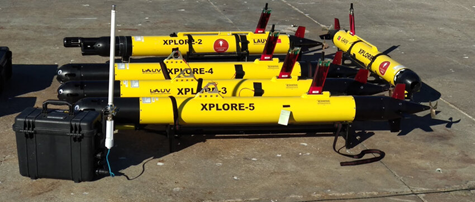
\includegraphics[width=.7\linewidth]{fig/lauvs.png}
    \caption{AUVs deployed in the \proj experiment.}
    \label{fig:lauvs}
\end{figure}

In-situ data collection process involved three upper water-column AUVs
(XP2, XP3 and XP5) which alternated daily in performing targeted
sampling missions over the \naz Canyon region. These vehicles designed
and developed in-house at the University of Porto \cite{sousa2012lauv}
came equipped with a range of sensors including a CTD
(Fig. \ref{fig:lauvs}). Some had in addition fluorometers, turbidity,
Oxygen, DVL/ADCP sensors while all came equipped with WiFi and Iridium
satellite communications, acoustic modems, and battery packs enabling
60h+ endurance; the CTDs mounted on the AUVs were cross-calibrated to
ensure consistency. In addition to the hardware involved, an extensive
suite of mature mission planning and command/control tools were used
-- discussion of these is outside the scope of the paper and can be
referenced at
\cite{dias2005neptus,seacons10,toolchain2012,pinto2013lsts,Ferreira2018}.

\kcomment{Ana, we need a paragraph, potentially with a figure on the
  asynchronous data assimilation in the statistical model from
  AUVs. Are any other sources (e.g. remote sensing) assimilated? If
  so, how so and with what frequency?}

% at IH calibration facilities. The
% Manta communication gateways \cite{} are equipped with acoustic
% modems, satellite and Wi-Fi modules for long range communications with
% underwater, surface, and aerial vehicles. The AUV operations were
% supported by two boats rented in Nazaré. In addition, to the existing
% command and control center located in Porto, LSTS installed another in
% Nazaré. Two Manta units were installed in the support boats to support
% local deployments and communications with the command and control
% centers. Four units were used to support the command and control
% center installed in Nazaré.

% \subsubsection{System of systems for ocean observation}

% TO DECIDE:
% \begin{itemize}
%     \item INCLUDE IH explaining that here we are focused on auv data
%     \item check for the definition of C2 for the first time
%     \item PRESENT EXAMPLES OF RIPPLES LAYERS HERE OR REFER TO OTHER SECTIONS WERE THOSE MAY BE DISPLAYED
%     \item INCLUDE MODEL AND MAKE OF SENSORS
% \end{itemize}

% The System of Systems for ocean observation deployed in this field study
% comprised systems contributed by the LSTS, the Hydrographic Institute
% (IH), Portuguese Navy, and the University of Columbia.

% IH deployed the NRP \emph{D. Carlos} oceanographic vessel contributing
% wet laboratories, a rosette equipped with CTDs, Niskin bottles and an
% Underwater Vision
% Profiler %(http://www.hydroptic.com/index.php/public/Page/product_item/UVP6-LP)%,
% and an Alseamar Glider equipped with a
% CTD %(https://www.alseamar-alcen.com/ocean-science-sector/seaexplorer-gliders/seaexplorer-1000/)%.

% LSTS deployed 5 Xplore long endurance AUVs along with 6 Manta
% communication gateways (Figure \ref{fig:lauvs}) and control stations for
% the field experiments in Nazaré. The Xplore class AUV \cite{lauvurl} is
% an AUV designed for water column operations equipped with CTD,
% fluorometer, turbidity, O2, cameras, and nutrient sensors, WiFi and
% satellite communications (Iridium), acoustic modems, and battery packs
% enabling 60h+ endurance. The CTDs mounted on the AUVs were calibrated
% and cross-calibrated at IH calibration facilities. The Manta
% communication gateways \cite{} are equipped with acoustic modems,
% satellite and Wi-Fi modules for long range communications with
% underwater, surface, and aerial vehicles. The AUV operations were
% supported by two boats rented in Nazaré. In addition, to the existing
% command and control center located in Porto, LSTS installed another in
% Nazaré. Two Manta units were installed in the support boats to support
% local deployments and communications with the command and control
% centers. Four units were used to support the command and control center
% installed in Nazaré.

% \begin{figure}
%     \centering
%     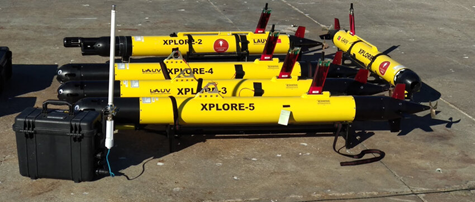
\includegraphics[width=.7\linewidth]{fig/lauvs.png}
%     \caption{The AUVs deployed in the experiment.}
%     \label{fig:lauvs}
% \end{figure}


% The Columbia University deployed a vertical profiler equipped with a CTD
% and portable CTD deployed from the support boats.

% The Xplore AUVs, control stations, and Manta gateways were powered by
% the LSTS software toolchain \cite{pinto2013lsts} deploying command and
% control, data pipelines, and algorithm integration to support closing
% the modeling-sample-assimilation-tasking cycles. The 4 components of the
% toolchain are briefly described below:

% DUNE, the onboard control software, running on vehicles and other
% devices. DUNE interfaces with sensors and actuators, by sending commands
% and monitoring them. DUNE is also in charge of executing missions and
% commands sent by the command and control (C2) stations. DUNE and its
% upper water column backseat implementation provided additional
% functionally for Iridium satellite communications, telemetry, and
% interaction with Neptus.

% IMC, the messaging protocol. It includes a definition of messages and
% its serialization. It is used to send and receive commands and data
% between vehicles and the C2 stations. A few IMC messages were created to
% support this field experiment. NEPTUS, the C2 software framework. Neptus
% presents a graphical user interface (GUI) enabling the operator to
% connect to one or several heterogeneous vehicles (underwater, surface,
% aerial, or sensors). With Neptus, one operator can control multiple
% vehicles simultaneously, sending commands, missions, and receiving and
% monitoring telemetry and data using Wi-Fi acoustics, or satellite
% communications. For this deployment Neptus incorporated new developments
% to streamline the integration of telemetry coming through the Iridium
% satellite communications with existing GUIs and to import optimal routes
% generated by the adaptive sampling algorithm into mission plans to send
% to the vehicles.

% RIPPLES, the Web based C2 that supports situational awareness of
% unmanned systems operations. It supports real-time monitoring of an
% operation and planning of such operations by providing access to several
% data products layers. These layers include environmental data and other
% support models for the environment and additions marine traffic in the
% vicinity of the operating autonomous vehicles (such AIS and aircraft
% data, or density maps). New layers were added to RIPPLES to support new
% aspects planning and execution control for this deployment.

% Figure XXX shows outputs of the HOPS (Harvard Ocean Prediction System)
% with temperature and salinity model outputs and respective errors.
% Another layer displayed geostatistical model outputs XXX. These outputs
% were used to monitor progress by enabling the visualization of updated
% during the execution of the operation.

% IH has several buoys in the area. A new layer to directly access and
% visualize their data in real-time was added to RIPPLES (Figure
% \ref{fig:buoys}. This provided wave information for the area (real-time
% and historical).


% \begin{figure}
%     \centering
%     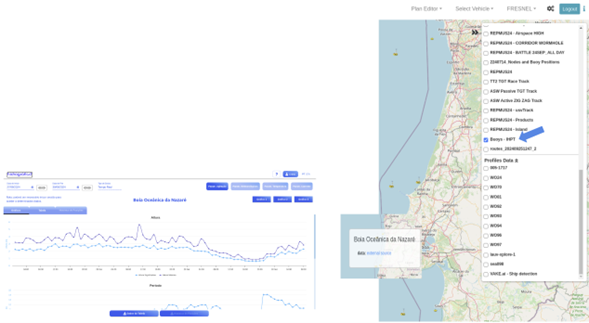
\includegraphics[width=.7\linewidth]{fig/buoys.png}
%     \caption{AUVs deployed in the experiment.}
%     \label{fibuoys}
% \end{figure}

 
% Optimal routes were generated for the AUVs to execute. A new Ripples
% layer enabled the user to visualize all the routes taken by the AUVs, as
% well as the routes generated for future deployments. This contributed to
% a timely launch and deployment of the vehicles.
 
% New layers for the visualization of remote sensing data, as well as of
% data collected by sensors installed onboard NRP D. Carlos were also
% deployed.


% The adaptive sampling problem is formulated as an optimization task
% aiming to maximize the expected information gain from the
% observations. Specifically, given the predicted uncertainty map and
% operational constraints (e.g., time, energy budget), the algorithm
% plans vehicle routes that prioritize areas of higher model
% uncertainty. The uncertainty along each candidate path is evaluated,
% and path planning strategies — such as greedy heuristics or
% combinatorial optimization techniques — are employed to allocate
% waypoints efficiently among the available AUVs.

% \subsubsection{Field deployment: planning and preparation}

% IH contributed the NRP D. Carlos for 5 days during one of the planned
% offshore buoy maintenance missions taking place annually in April or in
% October. The October period was selected for the \proj deployment. The
% meteorological and ocean conditions are typically not significantly
% different in these periods and may be affected by distant storms taking
% place in the Atlantic.

% The planned time window for the \proj deployment with NRP D. Carlos was
% the second week of October. However, this time window had to be shifted
% by one week, to start October 20th, because of challenging
% meteorological and ocean conditions. The AUV deployments were planned to
% start the first week of October but were delayed starting October 14th
% and end October 31st. The decisions to delay both the ship and AUV
% deployments proved to be adequate and made it possible to have 5 days of
% ship time and 7 days of AUV operations. This also enabled concurrent
% operations of the ship, glider, and AUVs. The AUVs collected data one
% week in advance of the ship’s arrival and kept running the developed
% algorithms during the third week of the deployment. The planned areas of
% operation for NRP D. Carlos (large rectangle) and for the AUVs (smaller
% rectangle) are depicted next.

% \begin{figure}
%     \centering
%     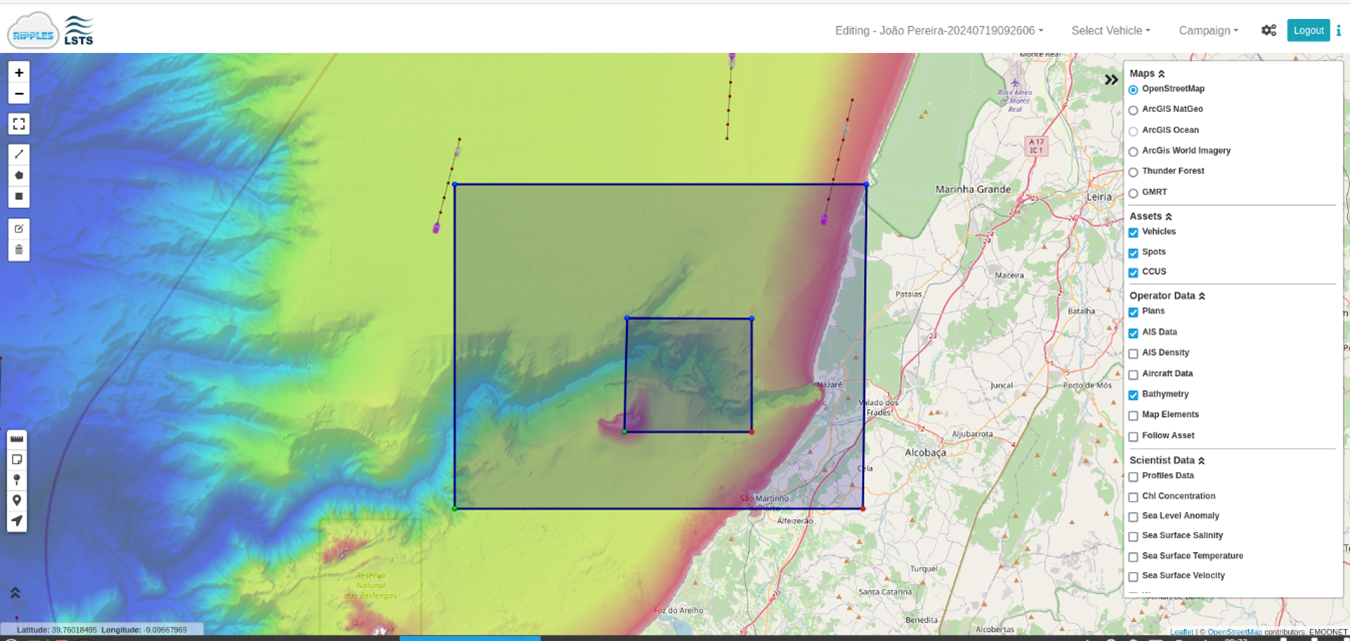
\includegraphics[width=.7\linewidth]{fig/Opareaas.png}
%     \caption{Areas of operations for NRP D. Carlos and for the AUVs.}
%     \label{fig:opareas}
% \end{figure}

% These areas have intense ship traffic, particularly from fishing
% vessels, that presents added collision risks to AUVs at surface or when
% surfacing, as well as potential encounters with bottom trawling fishing
% nets. In addition, because Nazaré is a fishing harbor there is the added
% challenge of AUV encounters with fishing nets.

% To address these challenges we started by meeting fisherman associations
% with the support of the city hall to engage the community, understand
% their fishing procedures and the probable locations of fishing nets.
% Second, we studied AIS patterns and densities, first for one year, then
% for one month, and finally for each week in October. This enabled us to
% partition the operations area into 3 areas with increasing risk levels
% \ref{fig:riskareas}. We focused our operations on the first two areas,
% starting operations at the one where risk was lower. Finally, by
% studying daily patterns we were able to establish temporary areas for
% operations with acceptable risks. We have distilled this knowledge into
% operational procedures and automated decision aids and alerts.

% \begin{figure}
%     \centering
%     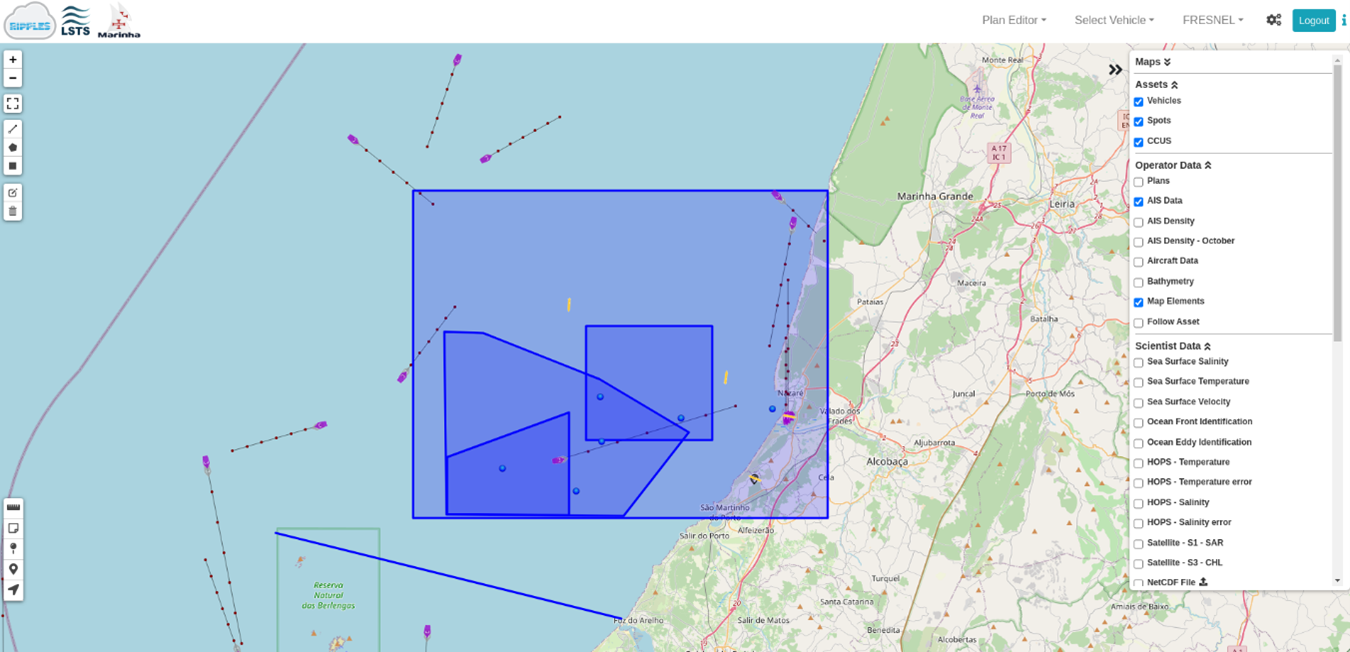
\includegraphics[width=.7\linewidth]{fig/riskareas.png}
%     \caption{The operational area was partitioned into 3 areas with
%       different levels of risk} XXX PLACE RISK MAP SIDE BY SIDE
%     \label{fig:riskareas}
% \end{figure}

% Field operations were organized into two concurrent activities:

% \begin{itemize}
% \item NRP \emph{D. Carlos} campaign taking place October 20th – 24th.
%   Team members from the University of Aveiro were onboard NRP D. Carlos
%   to support operations with the UVP and wet laboratory operations. In
%   addition to the rosette casts a glider was also deployed from the
%   ship. The deployment of the glider along the western boundary of the
%   operations area provided some of the initial conditions for the HOPS
%   model. The rosette casts provided a course description of essential
%   ocean variables in the larger area of operation. XXX Detailed
%   descriptions of these activities are presented in Annexes E - H.

% \item AUV deployments taking place October 14th - 31st. These
%   deployments were supported by two boats rented in Nazaré. In addition
%   to the AUV deployments by LSTS-UPorto, water samples were collected by
%   researchers from Columbia University. These data collection activities
%   provided a dense grip of data collection points. XXX Detailed
%   descriptions of these activities are presented in Annexes D, F, G.

% \end{itemize}

% These two activities were conducted in coordination, namely in what
% concerns water space management and sharing of model predictions, done
% with the help of the LSTS toolchain and the underlying communication
% infrastructure. Both activities run 24/x.

% In the case of the AUV deployments the LSTS-UPorto team operated in 4
% 6-hour long shifts with minimal operator’s footprint (one active and
% one backup operator).  Operations were run from a house rented in
% Nazaré and from LSTS in Porto.


% \subsubsection{Deployment and operations}

% Questions:
% \begin{itemize}
%     \item explain yoyos
%     \item include a more detailed description of daily ops with tables?
% \end{itemize}


% AUV daily operations started with the analysis of remote sensing data,
% data collected during the previous 24h, forecasts of meteorological and
% ocean condition, performance of the planning and execution control
% algorithms, performance of the modeling-sample-assimilation-tasking
% cycle (this was done during the last week of operations), and mission
% updates provided by the operators in charge of the night shifts.

% AUV operations’ planning then proceeded in 2 different time horizons:

% \begin{itemize}

% \item Plan for the day, including launch and recovery of
%   vehicles, as well as boat operations. 

% \item Plan for next 2-3 days (3 AUVs could operate for 50h+). This was
%   particularly challenging
%   because it included calculating time of recovery and making sure that
%   the meteorological and ocean conditions were feasible for these
%   operations. AUV execution control was focused on addressing alerts
%   (e.g., ships crossing the area of operations), coordinating launch and
%   recovery of AUVs with the help of the two boats, and re-tasking the
%   vehicles in case a significant change in the planning assumptions
%   occurred. 

% \end{itemize}

% \proj operations started spanned October 14th - 31st period. We took a
% risk-minimizing incremental approach to operations planning and
% execution control. The first week was about getting acquainted with the
% new area of operations and evaluating, testing, and improving
% operational procedures. The second week was about deploying the whole
% approach and learning from it. The third week focused on running AUV
% operations to further evaluate and test the approach, namely in what
% concerned simultaneous deployments and persistent observation.

% The first week was about AUV and small boat operations (including
% collecting water samples). The focus was on testing the validity of the
% risk management approach (including the partition of the operations
% area) and on evaluating and testing the operation of the AUVs in this
% new area. AUV missions were already spanning at least 2-day durations.

% The second week involved the 5-day long NRP \emph{D. Carlos} campaign
% together with AUV operations with boat support for launch and recovery
% and water sampling. Coordination of these concurrent operations involved
% water space management, to prevent collisions, and ingestion of data
% provided by the ship and AUVs for analysis and assimilation. The
% experience acquired during this week was invaluable and provided the
% templates for AUV operations taking place the following week. Over these
% two weeks the AUVs were impacted several times by strong vertical
% currents in areas of significant stratification. Our preliminary
% analysis pointed to internal waves as the most probable cause of these
% currents. The area is known for internal wave activity and remote
% sensing data provided evidence of the presence of internal waves during
% the same days.

% The final week focused on AUV operations only. Multi-day AUV deployments
% provided additional data about the modeling-sample-assimilation-tasking
% cycle (executed several times). In addition, AUVs were deployed
% concurrently not only in the area surveyed the previous week (to
% minimize risk) but also in areas with higher risk of collisions in which
% short time windows limited the duration of these deployments. This
% required tighter planning and execution control procedures for the two
% operators in charge of the concurrent operations. This is illustrated
% with mission plans depicted in Figure \ref{fig:missionplans}. One AUV
% was tasked to perform yo-yos along straight line (line in black) in an
% area in which trawlers run North-South transects, while two others
% performed the adaptive sampling algorithm further South in a safer area.
 
% \begin{figure}
%     \centering
%     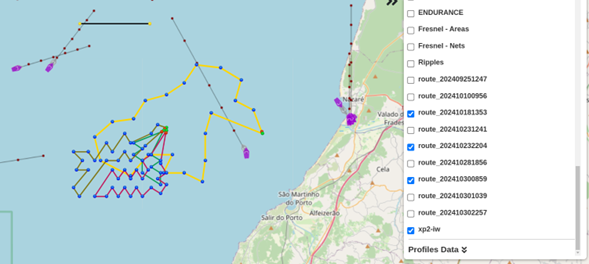
\includegraphics[width=.7\linewidth]{fig/missionplans.png}
%     \caption{Example of mission plans (tours) to be executed by 3 AUVs.}
%     \label{fig:missionplans}
% \end{figure}


% The AUV operators were provided with close to real-time information
% about the data collected by the AUVs, as depicted in Figure
% \ref{fig:temperatureprofiles} showing surfacing points for one mission
% color-coded by temperature. The operator could click in any of these
% points to get a temperature profile for the previous dive.

%  \begin{figure}
%     \centering
%     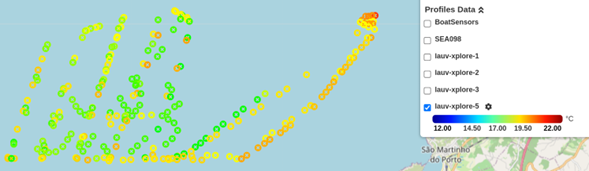
\includegraphics[width=.7\linewidth]{fig/temperatureprofiles.png}
%     \caption{AUV path color-coded by levels of temperature at surfacing points.}
%     \label{fig:temperatureprofiles}
% \end{figure}

% Despite the challenging meteorological and ocean conditions, that
% strongly constrained the overall deployment, the \proj team was able to
% demonstrate the overall approach during these 3 weeks (out of which only
% 7 days of operation were possible). The team operating the AUVs spent
% these 3 weeks on site and on call to rapidly deploy or recover the AUVs
% as dictated by meteorological and ocean conditions or forecasts.


Challenging meteorological and ocean conditions constrained the team
from multiple iterations of the
\emph{sample-assimilate-predict-direct} loop to
% Although the \proj field campaign extended over a longer period, for
% the purpose of this paper,
a three-day sequence of consecutive experiments (29-–31 October,
2025). The analysis in this work aims to quantify the impact of
assimilating AUV-acquired temperature data on the predictive
performance of the statistical model and to assess the operational
feasibility of the data cycle approach in a real-world coastal
setting. To simply the process the model's workflow and the
assimilation loop was focused only towards temperature data. As a
consequence this work is univariate in showing the impact of
assimilated model-driven exploration. We believe that results in Sec
\ref{sec:results} are general enough to apply to other critical
oceanographic variables which would need to be modeled similarly.

% is considered, as it provides a representative demonstration of
% the proposed framework and its operational workflow.

% The evaluation of the framework was carried out during the FRESNEL
% field campaign through a series of consecutive daily experiments
% designed to test the integration of model forecasts, target sampling
% planning, and data assimilation. All of these components were
% previously described. 
% The analysis aimed to quantify the impact of assimilating AUV-acquired
% temperature data on the predictive performance of the statistical
% model and to assess the operational feasibility of the data cycle
% approach in a real-world coastal setting.

Each experimental day followed a structured cycle involving: (i) the
generation of a statistical model forecast and its associated
uncertainty field based on the Copernicus Marine Service (CMS)
\cite{sotillo2021} data available up to the previous day; (ii) the
execution of the target sampling algorithm to plan the next-day
missions; and (iii) in situ data collection by AUVs following the
algorithmically determined transects. The data collected within the
previous day were subsequently assimilated into the statistical model
to produce updated forecasts, enabling comparisons between forecasts
with and without data assimilation.


\begin{figure}
    \centering
    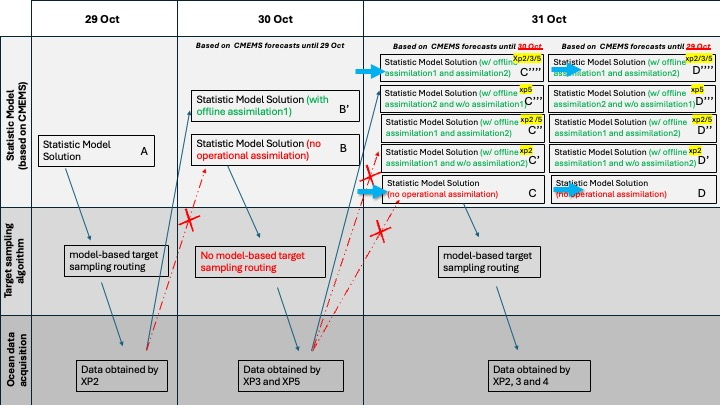
\includegraphics[scale=0.6]{fig/model-config.jpeg}
    \caption{The statistical model configurations and assimilation
      options used during the \proj experiment.}
    \label{fig:model-config}
\end{figure}

\kcomment{Renato, I think we might need to place a simplified version
  of figure from your powerpoint slide about the various
  configurations and versions of the models. I'm adding a version here
  which is probably old and too complicated. If you can do work on
  getting a simpler version which just shows what we used. The caption
  of the figure then will need to be explanatory.}

On 29\textsuperscript{th} October, the statistical model produced the
initial forecast solution (A), which was used to plan the mission
executed by XP2. The resulting in situ temperature data were later
assimilated offline to produce an updated statistical model solution
(B1) for 30 October. Although operational real-time assimilation was
initially planned, logistical constraints prevented its
implementation. Consequently, all assimilation cases were performed
offline after mission completion. The target sampling algorithm,
therefore, relied on statistical forecasts without assimilation (B),
using pre-existing data as input for daily mission planning. This
limitation is not expected to have significantly affected the
experimental outcomes, as the operational area was spatially compact
and the predicted variability field remained consistent between
consecutive days. In future implementations, on-board or
near-real-time assimilation should be considered to fully exploit the
adaptive potential of the framework.

Data collected by XP3 and XP5 on 30 October were assimilated offline
to generate new model solutions for 31 October (C1, C2, C3, C4), along
with a non-assimilated reference case (C). The configurations were as
follows:

\begin{itemize}
    \item C1 – assimilation including only XP2 data from 29 October;
    \item C2 – assimilation including XP2 (29 October) and XP5 (30 October) data;
    \item C3 – assimilation including only XP5 data from 30 October;
    \item C4 – assimilation including all available data from 29 and 30 October (XP2, XP3, and XP5).
\end{itemize}

An analogous setup was used for scenario D, in which the difference
from case C is that the statistical predictions for 31 October were
generated using CMS data available as prior up to different cutoff dates:

\begin{itemize}
    \item D – forecast for 31 October based on CMS data available as prior until 29 October;
    \item D1–D4 – corresponding to the same assimilation
      configurations as C1–C4, but using CMS data available as prior until 30
      October.
\end{itemize}

Model performance was evaluated by comparing predicted and observed
temperature data along the AUV trajectories using the root-mean-square
error (RMSE) as the primary performance metric for 31 October.

\begin{figure}
    \centering
    %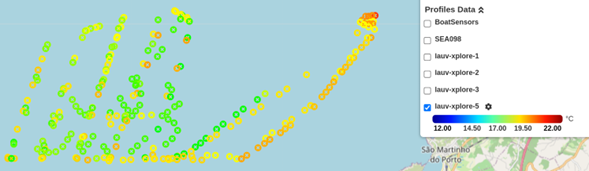
\includegraphics[width=.7\linewidth]{fig/temperatureprofiles.png}
    \caption{INSERT schematic about the 3-day loop}
    \label{fig:temperatureprofiles}
\end{figure}

% The practical implementation of the data cycle in a real-world marine environment introduces several constraints:

% \begin{itemize}
%
% \item \textbf{Communication Limitations}: Low-bandwidth and
%   intermittent communications at sea require that mission planning be
%   sufficiently robust to accommodate long periods of autonomous
%   operation without human intervention.
    
% \item \textbf{Vehicle Constraints}: AUV endurance, payload
%   limitations, navigation precision, and deployment risks all impose
%   restrictions on the feasible operational space and mission duration.

% \item \textbf{Computational Demands}: Real-time generation of
%   uncertainty fields, optimization of paths, and assimilation of
%   collected data must be performed within time windows compatible with
%   daily operational cycles, often under constrained computational
%   resources.

% \item \textbf{Environmental Variability}: Fast-evolving coastal ocean
%   dynamics can introduce discrepancies between forecasted and actual
%   conditions, necessitating robust planning that accounts for forecast
%   uncertainty and adaptivity. \end{itemize}

% This method was deployed and evaluated under the operational framework
% of the FRESNEL project, providing a real-world demonstration of the
% data cycle’s feasibility and benefits in complex coastal environments.


% Distinction Between Onboard and Offboard Predictions:
% \begin{itemize}
%     \item Onboard: Statistical prediction
%     \item Offboard: Numerical prediction
% \end{itemize}

% Rationale and Implementation (including a schematic figure):
% \begin{itemize}
%     \item Why this approach?
%     \item How was it executed?
% \end{itemize}

% Adaptive Sampling Strategy:
% \begin{itemize}
%     \item contraints
%     \item Algorithm used for real-time decision-making
%     \item Criteria for data collection optimization
% \end{itemize}

% Statistical Approach:
% \begin{itemize}
%     \item Techniques applied for uncertainty estimation
%     \item Integration with observational data
% \end{itemize}

%  Numerical Model (HOPS - Harvard Ocean Prediction System):
% \begin{itemize}
%     \item Model configuration and setup
%     \item Data assimilation methods
% \end{itemize}



\section{Results}
\textit{- Present your \textbf{findings} in a logical and coherent manner.}

\begin{itemize}
    \item Environmental context
    
\begin{figure}
    \centering
    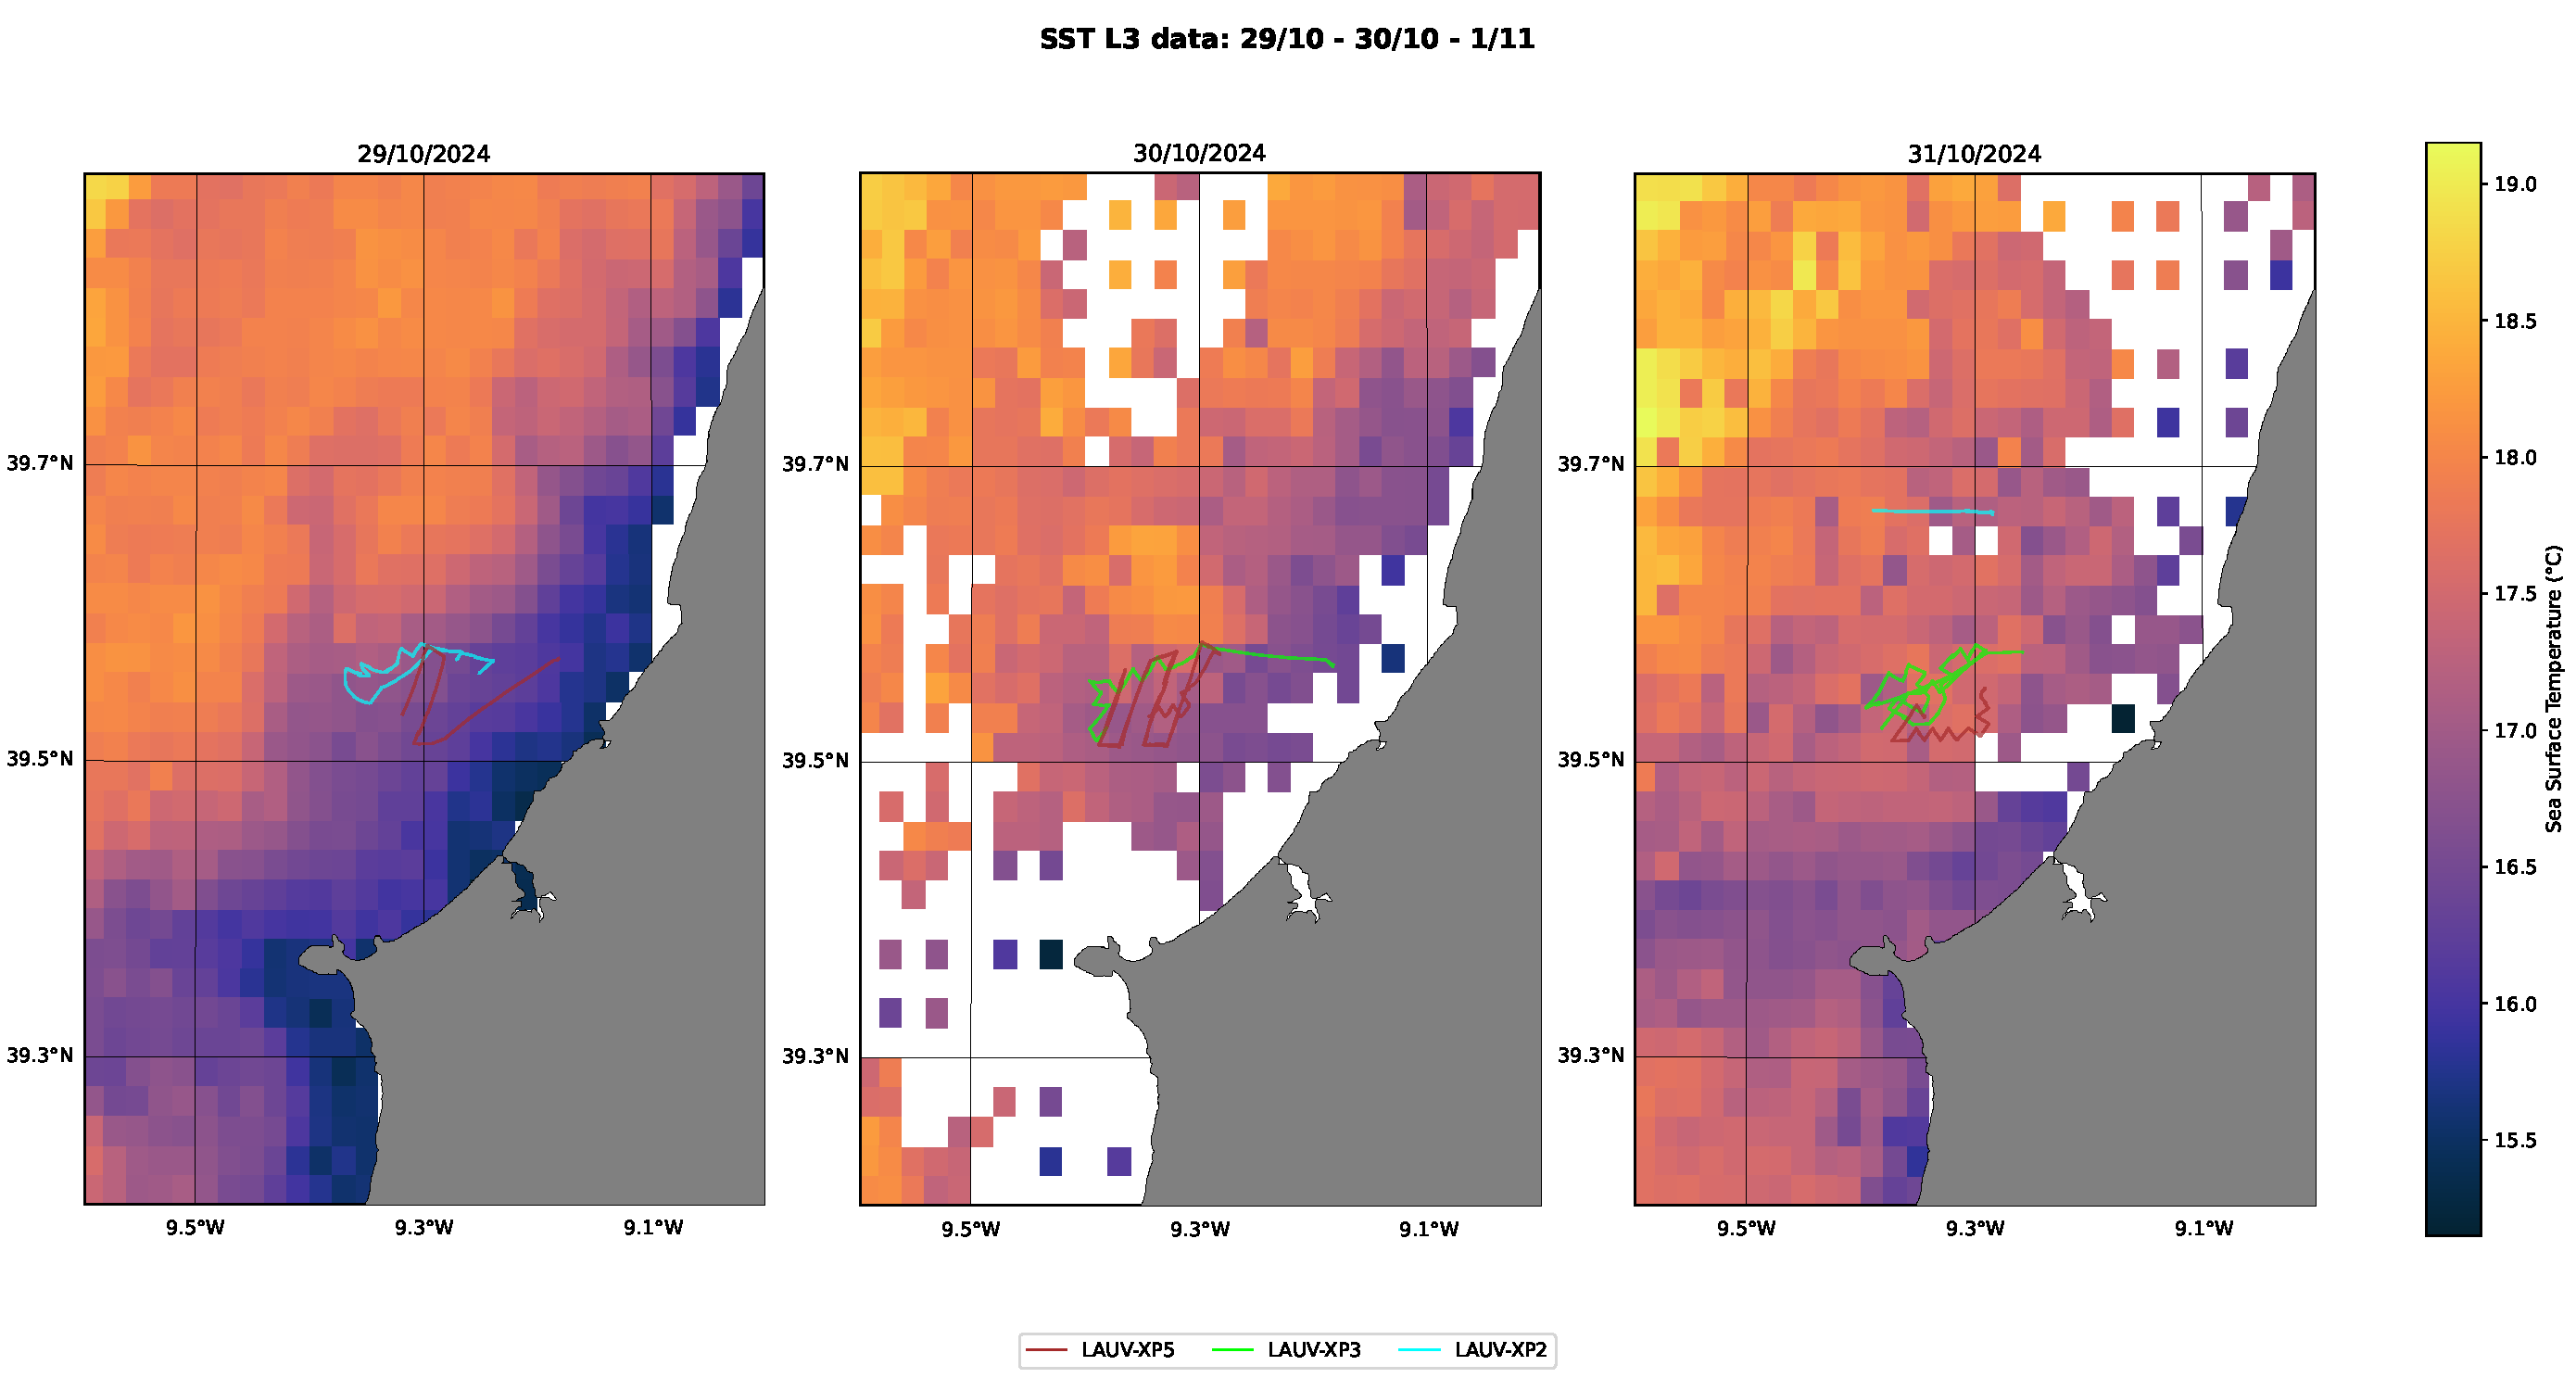
\includegraphics[width=1\linewidth]{fig/SST_L3_color1.pdf}
    \caption{L3 SST data + AUV trajectories over 3 days}
    \label{fig:temperatureprofiles}
\end{figure}

\begin{figure}
    \centering
    \includegraphics[width=1\linewidth]{fig/Figure2_100m.pdf}
    \caption{temperature data collected by AUV in depth (yy) over time (xx)}
    \label{fig:temperatureprofiles}
\end{figure}
    
    
    \item RMS table (all cases) + rms figure (just A+D cases)
\end{itemize}

 
\textit{- Use \textbf{subheadings} to organize different experiments or analyses.}

\section{Discussion}
\label{sec:disc}

The challenging ocean and meteorological conditions faced as part of
this experiment precluded cycles of week-long operations, as
planned. Nevertheless, we were able to operate for 7 days during the
3-week long deployment. We demonstrated the overall integrative
overall approach to close modeling-sampling-assimilation-tasking cycle
with the goal of improving the skill of oceanographic models by
leveraging observations from AUVs, traditional methods such as
ship-based measurements and opportunistic measurements using low-cost
sensors, and by exploring synergies between dedicated surveys and
opportunistic observations.

Full integration of command and control strategies comprising modeling,
assimilation and adaptive sampling algorithms was demonstrated with the
help of the advanced LSTS software toolchain enabling 24/x operations
with minimal operator’s support. The deployments were performed to
evaluate and test the overall approach in an incremental fashion. The
last days of the deployment demonstrated several iterations of the
closed modeling-sampling-assimilation-tasking cycle. The accuracy of the
predictions of the geostatistical model increased after several cycles,
while the overall prediction errors decreased. However, these results
still lack statistical significance because of the few consecutive
cycles in which the overall approach was tested. We observed that we
never had more than 3 consecutive days of operation.

The dense grid of AUV observations enables post-experiment evaluation
and testing of the assimilation schemes and of the geostatistical model.
While we are still lacking the desired statistical significance of a
long series of consecutive cycles, these post-experiment activities will
lead to a better understanding of the overall procedures and the
identification of improvements, namely the optimization of the
parameters used for the coordinated integration of the algorithms used
in the modeling-sample-assimilation-tasking cycles. We will further
investigate the selection of representative depths for the application
of the sampling algorithm used to find the horizontal projection of the
AUV paths.

This field study provided invaluable lessons in operational procedures,
refinement of adaptive sampling and algorithms, and risk minimization to
operate in an area with dense ship traffic and fishing nets. Our AUVs
were occasionally impacted by strong vertical currents that may have
resulted from the impact of internal waves that are common in the area,
namely in stratified regions (which was the case) and that were observed
with the help of remote sensing imagery during the deployments. Finally,
the results achieved with this deployment provided additional insights
and the motivation to further advance the state of the art in refining
the modeling-sampling-assimilation-tasking cycle with the goal of
improving the skill of oceanographic models. Furthermore, dense grids of
sampled oceanographic data have the potential to fuel developments
targeting existing gaps in modeling skill when different levels of
spatial and temporal resolution are considered \cite{Balaji_2022}.


\begin{figure}[!]
  \centering
  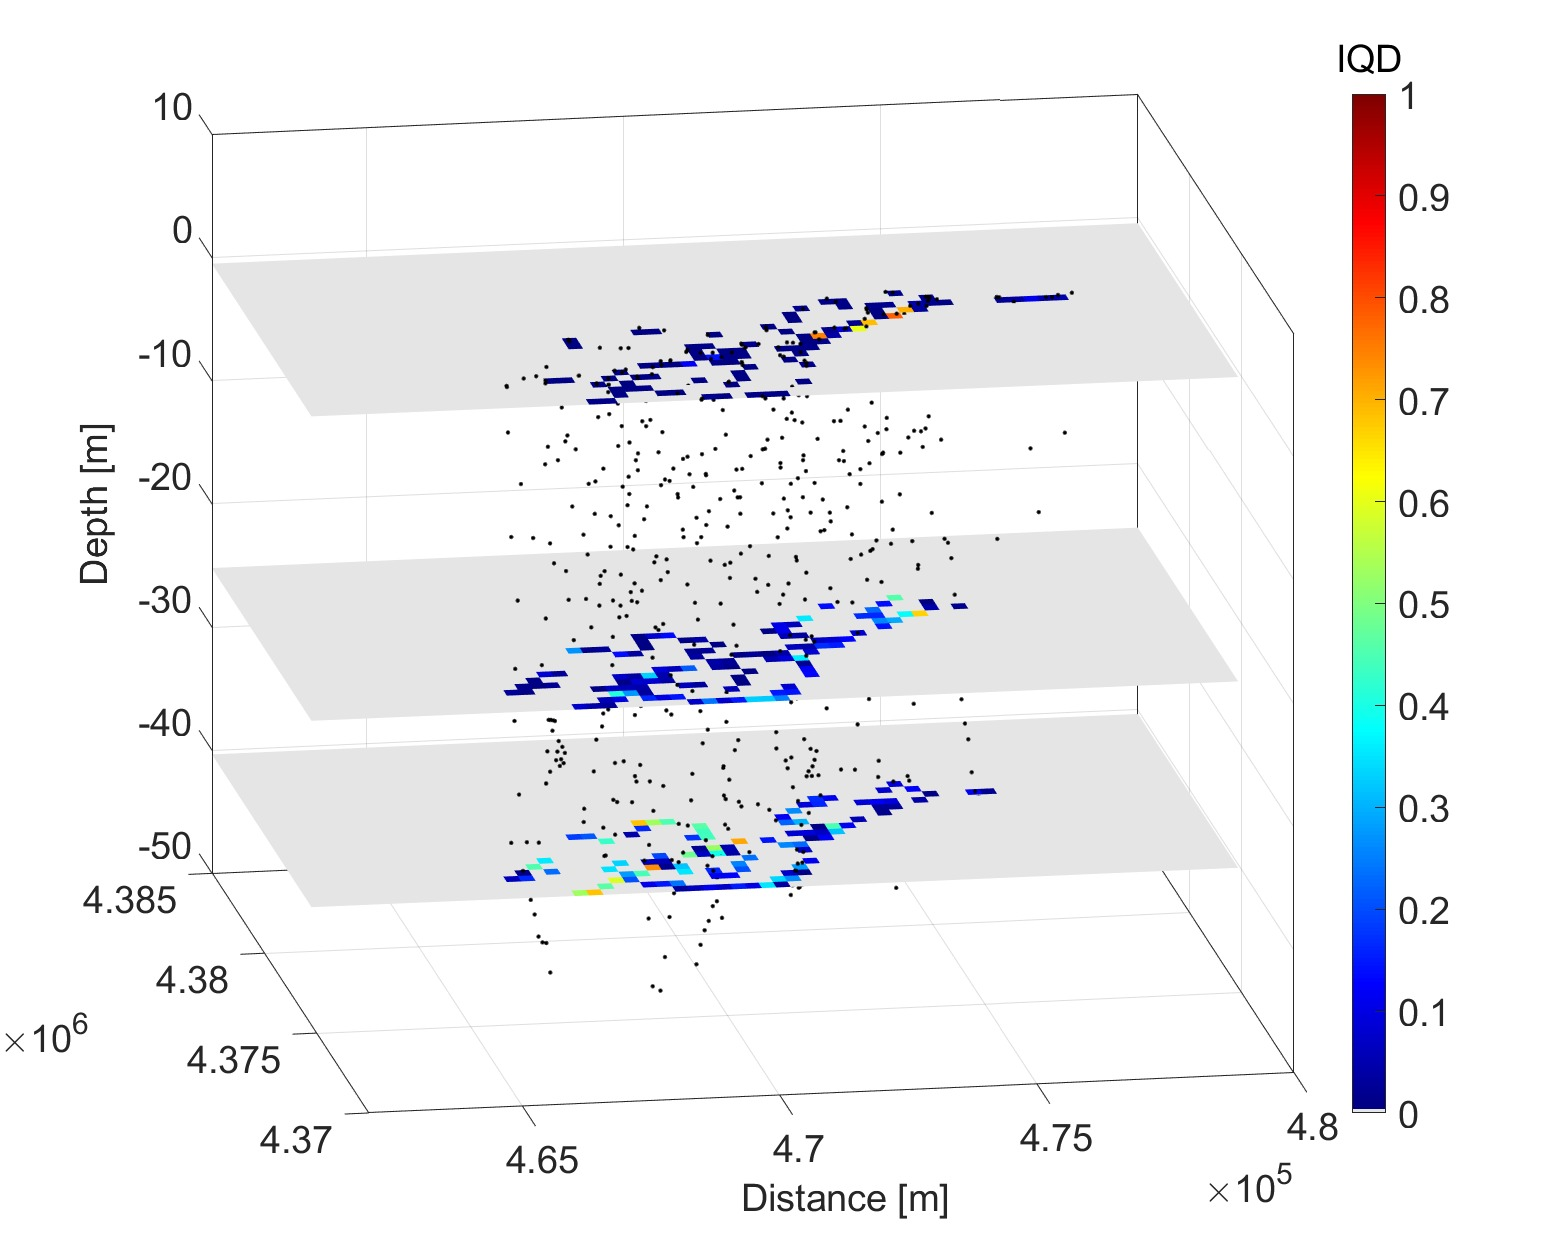
\includegraphics[scale=0.3]{fig/iqd_3D.jpeg}
  \caption{not the final figure}
  \label{fig:iqd_3D}
\end{figure}




\section{Acknowledgements}

This work was carried out with the support of the US Office of Naval
Research (ONR) contract \#:YYYY. We are grateful to Dr. Tom Drake
(Code 32) for his support. 

\bibliographystyle{IEEEtran}
\footnotesize{
  \bibliography{ref}
}
\end{document} 
